\documentclass[tikz, dvipsnames]{standalone}
\begin{document}
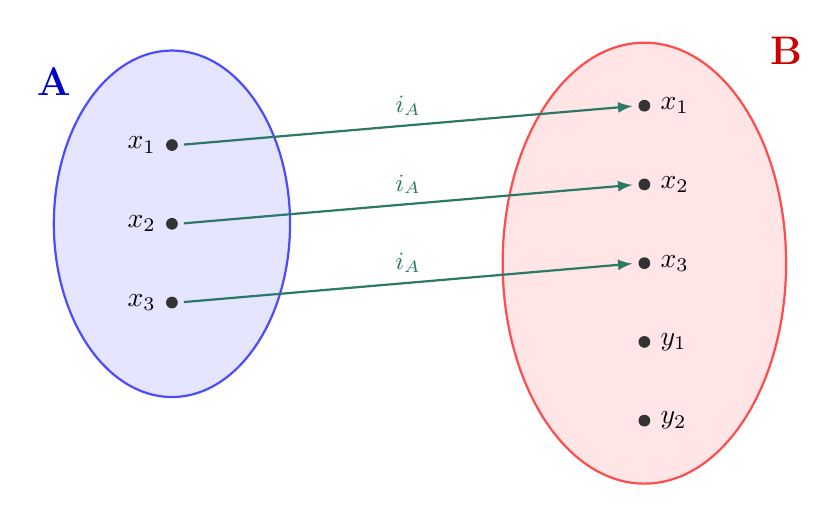
\begin{tikzpicture}[>=latex]

% --- Global TikZ Styles for Consistency ---
\tikzset{
    setA/.style={fill=blue!10, draw=blue!70, thick},
    setB/.style={fill=red!10, draw=red!70, thick},
    labelA/.style={text=blue!80!black, font=\Large\bfseries},
    labelB/.style={text=red!80!black, font=\Large\bfseries},
    point/.style={circle, fill=black!80, inner sep=1.5pt},
    arrow/.style={->, >=latex, thick, draw=black!60, shorten >=2pt, shorten <=2pt},
    mapLabel/.style={text=PineGreen!80!black, font=\small\bfseries}
}

    % Verzameling A
    \path[setA] (0, 1.0) ellipse (1.5cm and 2.2cm);
    \node[labelA] at (-1.5, 2.8) {A};

    % Elemeten van A
    \node[point, label=left:$x_1$] (a1) at (0, 2.0) {};
    \node[point, label=left:$x_2$] (a2) at (0, 1.0) {};
    \node[point, label=left:$x_3$] (a3) at (0, 0.0) {};

    % Verzameling B
    \path[setB] (6, 0.5) ellipse (1.8cm and 2.8cm);
    \node[labelB] at (7.8, 3.2) {B};

    % Elementen van B
    \node[point, label=right:$x_1$] (b1) at (6, 2.5) {};
    \node[point, label=right:$x_2$] (b2) at (6, 1.5) {};
    \node[point, label=right:$x_3$] (b3) at (6, 0.5) {};

    \node[point, label=right:$y_1$] (b4) at (6, -0.5) {};
    \node[point, label=right:$y_2$] (b5) at (6, -1.5) {};

    % Pijlen
    \draw[arrow, draw=PineGreen!80!black] (a1.east) -- node[above, mapLabel] {$i_A$} (b1.west);
    \draw[arrow, draw=PineGreen!80!black] (a2.east) -- node[above, mapLabel] {$i_A$} (b2.west);
    \draw[arrow, draw=PineGreen!80!black] (a3.east) -- node[above, mapLabel] {$i_A$} (b3.west);

    
\end{tikzpicture}
    
\end{document}